% FreeToken4GB Visual Guide — the picture book for humans (and LLMs who read .tex)
% Regenerate: make -C docs/visual   (requires pdflatex + latexmk + tikz/pgfplots)
\documentclass[11pt,a4paper]{article}
\usepackage{geometry}
\geometry{margin=2.2cm}
\usepackage{amsmath}
\usepackage{tikz}
\usepackage{pgfplots}
\pgfplotsset{compat=1.18}
\usetikzlibrary{arrows.meta,positioning,shapes.geometric,calc,fit,backgrounds}
\usepackage{xcolor}
\usepackage{booktabs}
\usepackage[colorlinks=true,linkcolor=blue!60!black,urlcolor=blue!60!black]{hyperref}

\definecolor{gpu}{RGB}{31,119,180}
\definecolor{cpu}{RGB}{255,127,14}
\definecolor{kv}{RGB}{44,160,44}
\definecolor{bad}{RGB}{214,39,40}
\definecolor{park}{RGB}{148,103,189}

\newcommand{\MiB}[1]{#1\,MiB}

\title{\textbf{FreeToken on 4\,GiB — The Picture Book}\\
\large Qwen3.6-35B-A3B-NVFP4 on an RTX 3050 Laptop, in diagrams}
\author{FreeToken4GB fork — visual companion to \texttt{docs/}}
\date{2026-09-14}

\begin{document}
\maketitle
\tableofcontents

%=====================================================================
\section{You are here: the reading map}
%=====================================================================
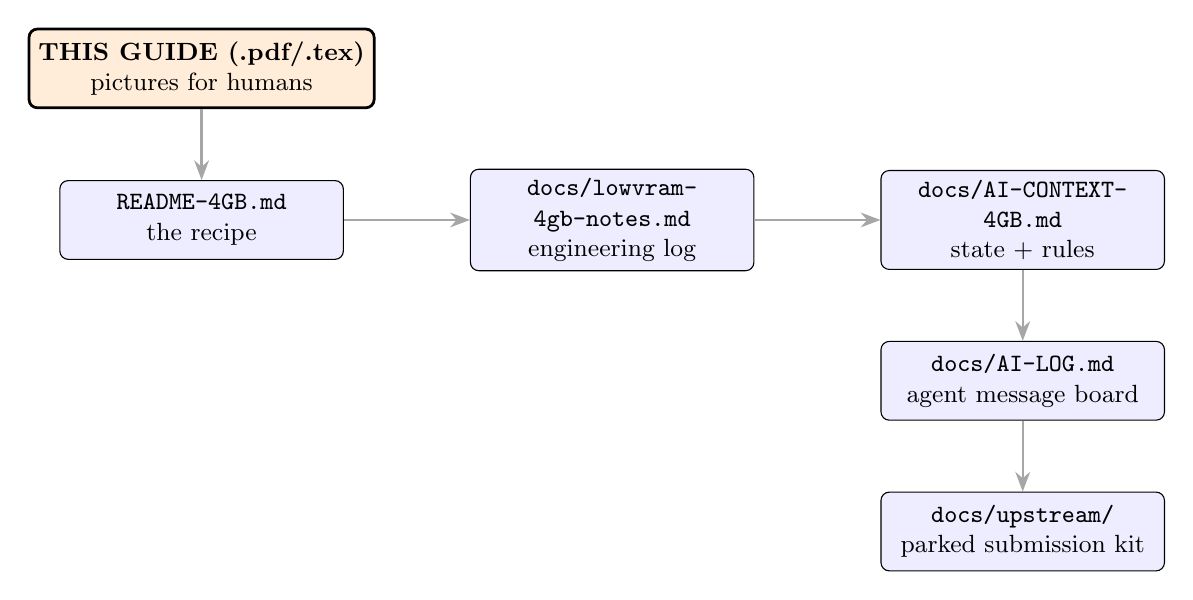
\begin{tikzpicture}[
  node distance=0.9cm and 1.6cm,
  doc/.style={draw, rounded corners=3pt, fill=blue!7, minimum width=3.6cm,
              minimum height=1.0cm, align=center, font=\small},
  vis/.style={doc, fill=orange!15, line width=1pt},
  arrow/.style={-{Stealth[length=2.5mm]}, thick, gray!70}]
  \node[vis] (this) {\textbf{THIS GUIDE (.pdf/.tex)}\\pictures for humans};
  \node[doc, below=of this] (readme) {\texttt{README-4GB.md}\\the recipe};
  \node[doc, right=of readme] (notes) {\texttt{docs/lowvram-}\\ \texttt{4gb-notes.md}\\engineering log};
  \node[doc, right=of notes] (aictx) {\texttt{docs/AI-CONTEXT-}\\ \texttt{4GB.md}\\state + rules};
  \node[doc, below=of aictx] (ailog) {\texttt{docs/AI-LOG.md}\\agent message board};
  \node[doc, below=of ailog] (upst) {\texttt{docs/upstream/}\\parked submission kit};
  \draw[arrow] (this) -- (readme);
  \draw[arrow] (readme) -- (notes);
  \draw[arrow] (notes) -- (aictx);
  \draw[arrow] (aictx) -- (ailog);
  \draw[arrow] (ailog) -- (upst);
\end{tikzpicture}

\medskip
Each layer adds detail: the recipe says \emph{what to run}; the notes say
\emph{why it works and what was measured}; the AI files say \emph{where the
project stands and what is next}.

%=====================================================================
\section{The budget problem: why 4\,GiB was ``impossible''}
%=====================================================================
Stock FreeToken 0.1.2 needs more than the card has. With everything in BF16:

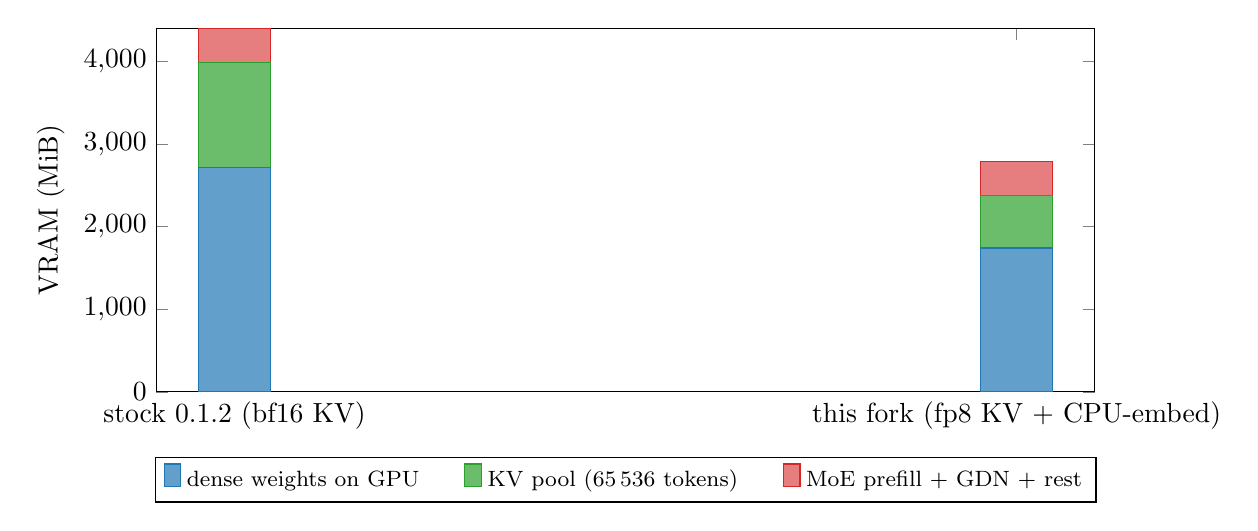
\begin{tikzpicture}
\begin{axis}[
  width=13.5cm, height=6.2cm,
  ybar stacked, bar width=26pt,
  ymin=0, ymax=4400,
  ylabel={VRAM (MiB)},
  symbolic x coords={stock 0.1.2 (bf16 KV), this fork (fp8 KV + CPU-embed)},
  xtick=data, x tick label style={align=center},
  legend style={at={(0.5,-0.18)}, anchor=north, legend columns=3,
                font=\footnotesize, /tikz/every even column/.append style={column sep=0.5cm}},
  nodes near coords style={font=\tiny}, every node near coord/.append style={color=white}]
\addplot+[gpu, fill=gpu!70] coordinates {
  (stock 0.1.2 (bf16 KV),2714) (this fork (fp8 KV + CPU-embed),1741)};
\addplot+[kv, fill=kv!70] coordinates {
  (stock 0.1.2 (bf16 KV),1270) (this fork (fp8 KV + CPU-embed),635)};
\addplot+[bad, fill=bad!60] coordinates {
  (stock 0.1.2 (bf16 KV),410) (this fork (fp8 KV + CPU-embed),410)};
\legend{dense weights on GPU, KV pool (65\,536 tokens), MoE prefill + GDN + rest}
\end{axis}
\end{tikzpicture}

\medskip
Stock: $2714+1270+410 \approx \mathbf{4394}$\,MiB $>$ 4096 — over the card before
CUDA-graph scratch. This fork: embedding table (\MiB{970}) moved to CPU and KV
halved to FP8 fits with \textbf{717.8\,MiB to spare} after full init.

%=====================================================================
\section{Where the model lives: the two-machine-in-one view}
%=====================================================================
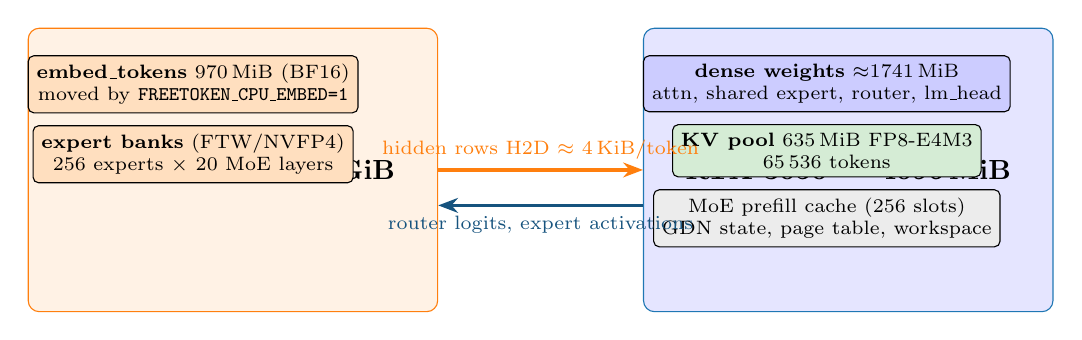
\begin{tikzpicture}[
  comp/.style={draw, rounded corners=4pt, minimum width=5.2cm, minimum height=3.6cm},
  part/.style={draw, rounded corners=2pt, align=center, font=\scriptsize, inner sep=3pt},
  ann/.style={font=\tiny, text width=2.6cm, align=center},
  arrow/.style={-{Stealth[length=2.5mm]}, very thick}]

\node[comp, fill=orange!10, draw=cpu] (host) {\textbf{HOST RAM — 32\,GiB}};
\node[part, fill=orange!25, below=0.35cm of host.north west, anchor=north west]
  (embed) {\textbf{embed\_tokens} 970\,MiB (BF16)\\moved by \texttt{FREETOKEN\_CPU\_EMBED=1}};
\node[part, fill=orange!25, below=0.15cm of embed]
  (banks) {\textbf{expert banks} (FTW/NVFP4)\\256 experts $\times$ 20 MoE layers};

\node[comp, fill=blue!10, draw=gpu, right=2.6cm of host] (gpu) {\textbf{RTX 3050 — 4096\,MiB}};
\node[part, fill=blue!20, below=0.35cm of gpu.north west, anchor=north west]
  (dense) {\textbf{dense weights} $\approx$1741\,MiB\\attn, shared expert, router, lm\_head};
\node[part, fill=kv!20, below=0.15cm of dense]
  (kv) {\textbf{KV pool} 635\,MiB FP8-E4M3\\65\,536 tokens};
\node[part, fill=gray!15, below=0.15cm of kv]
  (rest) {MoE prefill cache (256 slots)\\GDN state, page table, workspace};

\draw[arrow, cpu] (host.east) -- node[above, font=\scriptsize, sloped]
  {hidden rows H2D $\approx$ 4\,KiB/token} (gpu.west);
\draw[arrow, gpu!70!black] (gpu.west) ++(0,-0.45cm) -- node[below, font=\scriptsize, sloped]
  {router logits, expert activations} ($(host.east)+(0,-0.45cm)$);
\end{tikzpicture}

\medskip
Decode MoE runs on 8 CPU threads pinned to cores 0--3; the GPU keeps attention,
the dense path and sampling. One card, two brains.

%=====================================================================
\section{One decode step: the token's journey}
%=====================================================================
\resizebox{\textwidth}{!}{%
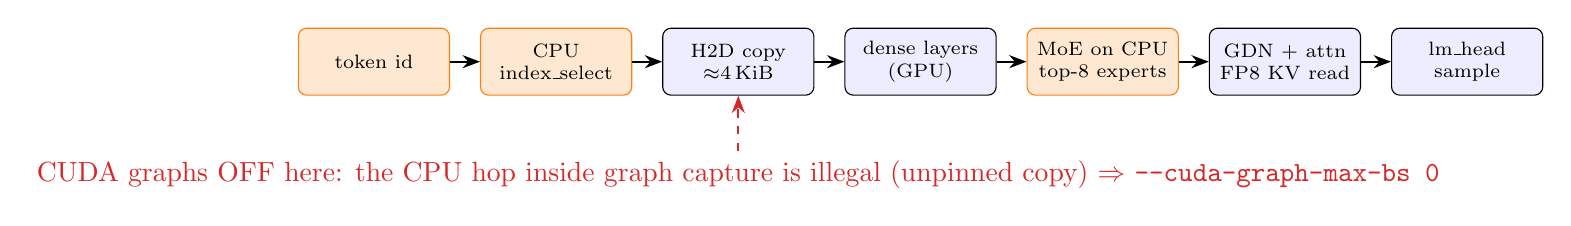
\begin{tikzpicture}[
  node distance=0.38cm,
  stp/.style={draw, rounded corners=3pt, fill=blue!7, minimum width=1.92cm,
               minimum height=0.85cm, align=center, font=\scriptsize},
  hoststep/.style={stp, fill=orange!18, draw=cpu},
  arrow/.style={-{Stealth[length=2.2mm]}, thick}]

\node[hoststep] (tok) {token id};
\node[hoststep, right=of tok] (emb) {CPU\\index\_select};
\node[stp, right=of emb] (h2d) {H2D copy\\$\approx$4\,KiB};
\node[stp, right=of h2d] (dense) {dense layers\\(GPU)};
\node[hoststep, right=of dense] (moe) {MoE on CPU\\top-8 experts};
\node[stp, right=of moe] (attn) {GDN + attn\\FP8 KV read};
\node[stp, right=of attn] (head) {lm\_head\\sample};

\draw[arrow] (tok) -- (emb);
\draw[arrow] (emb) -- (h2d);
\draw[arrow] (h2d) -- (dense);
\draw[arrow] (dense) -- (moe);
\draw[arrow] (moe) -- (attn);
\draw[arrow] (attn) -- (head);

\node[bad, below=0.7cm of h2d, minimum width=3.2cm] (warn)
  {CUDA graphs OFF here: the CPU hop inside graph capture is illegal
   (unpinned copy) $\Rightarrow$ \texttt{-{}-cuda-graph-max-bs 0}};
\draw[arrow, bad, dashed] (warn.north) -- (h2d.south);
\end{tikzpicture}}

\medskip
The CPU embedding lookup and the CPU expert compute each cross PCIe once per
token — cheap next to reading 8 expert weight sets. Measured decode:
\textbf{10--14 tok/s} even at 65K context.

%=====================================================================
\section{The four changes, at a glance}
%=====================================================================
\begin{tikzpicture}[
  cell/.style={draw, rounded corners=3pt, fill=blue!6, text width=6.55cm,
               minimum height=2.6cm, align=left, font=\scriptsize, inner sep=5pt},
  arrow/.style={-{Stealth[length=2mm]}, very thick}]
\node[cell] (a) at (0,0) {
  \textbf{1. KV dtype $\to$ FP8-E4M3} \texttt{-{}-kv-dtype fp8\_e4m3}\\[2pt]
  \begin{tikzpicture}[font=\tiny]
    \draw[fill=kv!60] (0,0) rectangle (1.3,0.5); \node at (0.65,0.25) {bf16};
    \node at (1.75,0.25) {$\to$};
    \draw[fill=kv!30] (2.2,0) rectangle (2.85,0.5); \node[right] at (2.9,0.25) {fp8};
  \end{tikzpicture}\\
  KV cell halves: 635 vs 1270\,MiB @ 64K tokens. Compute stays BF16
  (\texttt{q\_dtype} split through flashinfer).};
\node[cell] (b) at (7.05,0) {
  \textbf{2. CPU embedding} \texttt{FREETOKEN\_CPU\_EMBED=1}\\[2pt]
  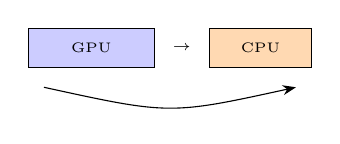
\begin{tikzpicture}[font=\tiny]
    \draw[fill=blue!20] (0,0) rectangle (1.6,0.5); \node at (0.8,0.25) {GPU};
    \node at (1.95,0.25) {$\to$};
    \draw[fill=orange!30] (2.3,0) rectangle (3.6,0.5); \node at (2.95,0.25) {CPU};
    \draw[-{Stealth}] (0.2,-0.25) .. controls (1.8,-0.6) .. (3.4,-0.25);
  \end{tikzpicture}\\
  970\,MiB table to host RAM; lookup there, 4\,KiB row back.\\
  \textcolor{bad}{Requires CUDA graphs OFF.}};
\node[cell] (c) at (0,-3.2) {
  \textbf{3. MoE cache fix} \texttt{-{}-moe-cache-size 256}\\[2pt]
  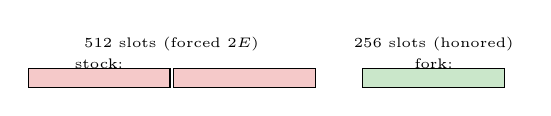
\begin{tikzpicture}[font=\tiny]
    \node at (0.9,0.3) {stock:};
    \draw[fill=bad!25] (0,0) rectangle (1.8,0.24);
    \draw[fill=bad!25] (1.85,0) rectangle (3.65,0.24);
    \node at (1.82,0.55) {512 slots (forced $2E$)};
    \node at (5.15,0.3) {fork:};
    \draw[fill=kv!25] (4.25,0) rectangle (6.05,0.24);
    \node at (5.15,0.55) {256 slots (honored)};
  \end{tikzpicture}\\
  Explicit size was silently doubled + overlap forced back on.\\
  See the parked upstream fix: \texttt{docs/upstream/}.};
\node[cell] (d) at (7.05,-3.2) {
  \textbf{4. Workspace right-sizing}\\[2pt]
  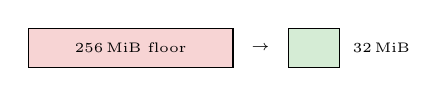
\begin{tikzpicture}[font=\tiny]
    \draw[fill=bad!20] (0,0) rectangle (2.6,0.5); \node at (1.3,0.25) {256\,MiB floor};
    \node at (2.95,0.25) {$\to$};
    \draw[fill=kv!20] (3.3,0) rectangle (3.95,0.5); \node[right] at (4.0,0.25) {32\,MiB};
  \end{tikzpicture}\\
  flashinfer workspace floor derived from TP-local geometry + SM count.
  Saves $\approx$224\,MiB on 20-SM cards, no behavior change.};
\end{tikzpicture}

%=====================================================================
\section{Memory ledger: every init checkpoint}
%=====================================================================
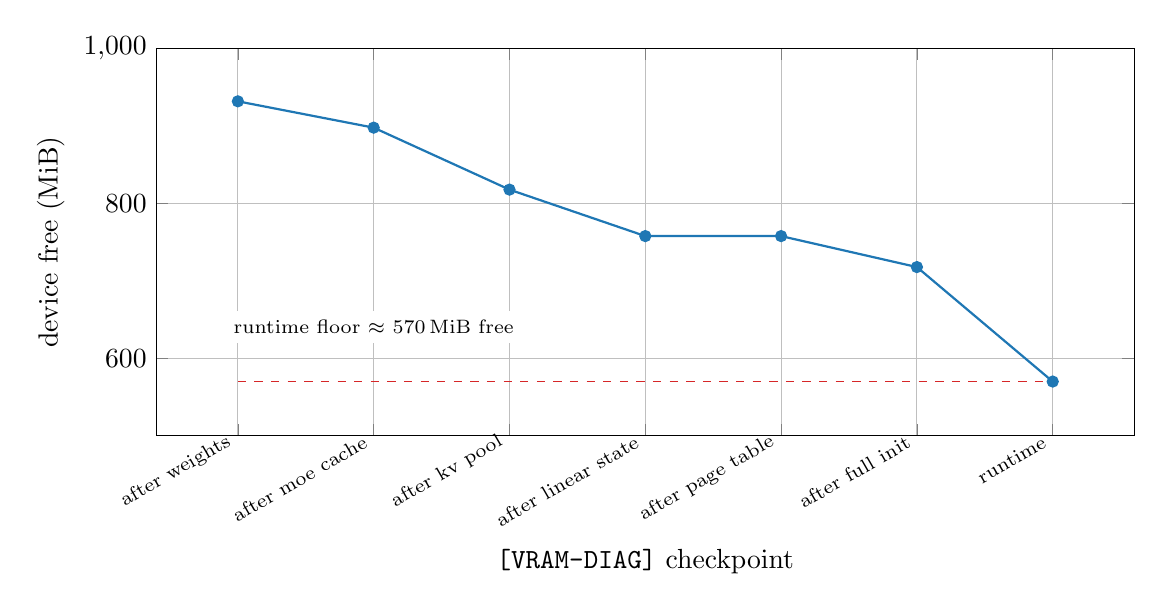
\begin{tikzpicture}
\begin{axis}[
  width=14cm, height=6.5cm,
  xlabel={\texttt{[VRAM-DIAG]} checkpoint},
  ylabel={device free (MiB)},
  ymin=500, ymax=1000,
  xtick={1,...,7},
  xticklabels={after weights, after moe cache, after kv pool,
               after linear state, after page table, after full init, runtime},
  x tick label style={rotate=30, anchor=east, font=\scriptsize},
  grid=major]
\addplot[color=gpu, thick, mark=*, mark size=1.8pt] coordinates {
  (1,931.8) (2,897.8) (3,817.8) (4,757.8) (5,757.8) (6,717.8) (7,570)};
\addplot[color=bad, dashed, no marks] coordinates {(1,570) (7,570)};
\node[font=\scriptsize, fill=white] at (axis cs:2,640)
  {runtime floor $\approx$ 570\,MiB free};
\end{axis}
\end{tikzpicture}

\medskip
Big steps: weights ($-3165$ incl. embed before offload), KV pool $-635$
(FP8!), GDN linear state $-60$, init tail $-40$. This chart is exactly what
\texttt{\_vram\_diag} prints — the diagnostic that found the 970\,MiB
embedding and the $256\to512$ cache doubling.

%=====================================================================
\section{Measured performance}
%=====================================================================
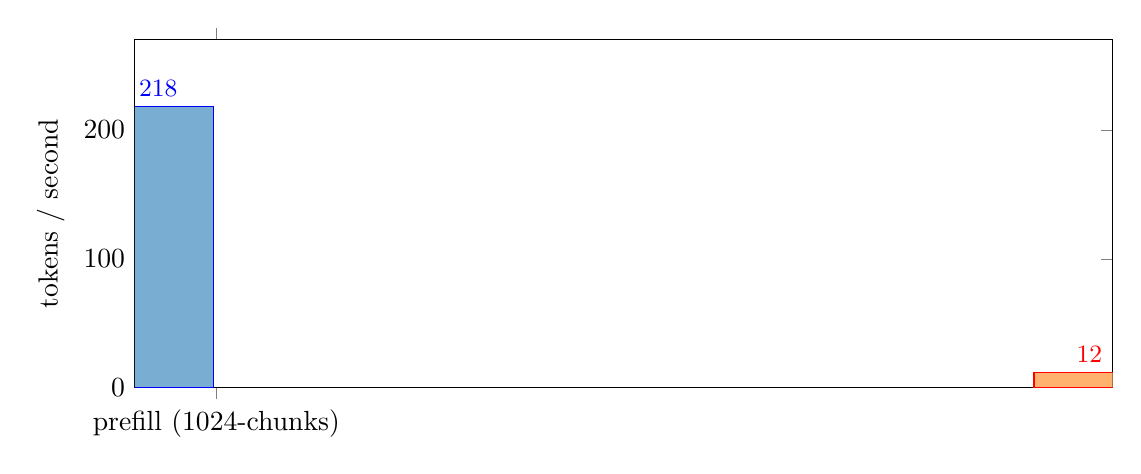
\begin{tikzpicture}
\begin{axis}[
  width=14cm, height=6cm,
  ybar, bar width=40pt,
  ymin=0, ymax=270,
  ylabel={tokens / second},
  symbolic x coords={prefill (1024-chunks), decode @ 10K--65K ctx},
  xtick=data,
  nodes near coords={\pgfmathprintnumber\pgfplotspointmeta},
  every node near coord/.append style={font=\small}]
\addplot+[fill=gpu!60] coordinates {(prefill (1024-chunks),218)};
\addplot+[fill=cpu!60] coordinates {(decode @ 10K--65K ctx,12)};
\end{axis}
\end{tikzpicture}

\medskip
Prefill 206--230 tok/s (first chunk per request is warm-up at 5--50);
decode 10--14 tok/s dominated by expert reads over PCIe. Soak test:
one request grew to \textbf{65,349 tokens} of combined context — pool usage
1.00, no OOM, no quality collapse.

%=====================================================================
\section{When it breaks: symptom $\to$ cause $\to$ fix}
%=====================================================================
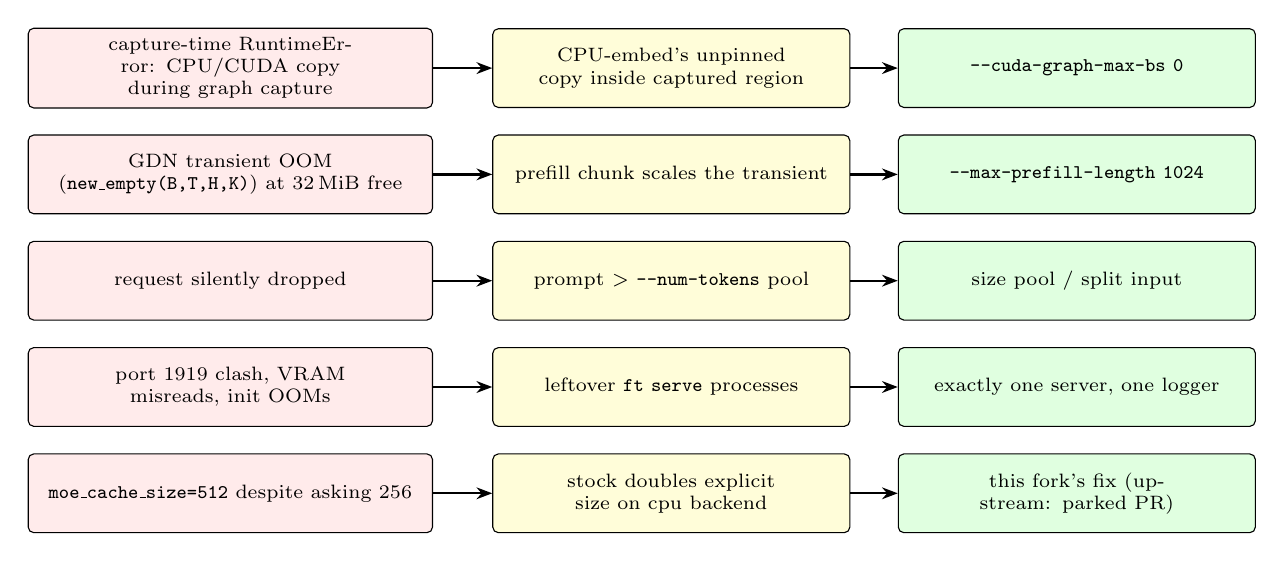
\begin{tikzpicture}[
  sym/.style={draw, rounded corners=2pt, fill=red!8, text width=4.9cm,
              align=center, font=\scriptsize, minimum height=1.0cm},
  cause/.style={draw, rounded corners=2pt, fill=yellow!15, text width=4.3cm,
              align=center, font=\scriptsize, minimum height=1.0cm},
  fix/.style={draw, rounded corners=2pt, fill=green!12, text width=4.3cm,
              align=center, font=\scriptsize, minimum height=1.0cm},
  arrow/.style={-{Stealth[length=2mm]}, thick}]
\def\row#1#2#3#4{%
  \node[sym]  (s#1) at (0,  -#1*1.35) {#2};
  \node[cause](c#1) at (5.6,-#1*1.35) {#3};
  \node[fix]  (f#1) at (10.75,-#1*1.35) {#4};
  \draw[arrow] (s#1) -- (c#1); \draw[arrow] (c#1) -- (f#1);}
\row{1}{capture-time RuntimeError: CPU/CUDA copy during graph capture}{CPU-embed's unpinned copy inside captured region}{\texttt{-{}-cuda-graph-max-bs 0}}
\row{2}{GDN transient OOM (\texttt{new\_empty(B,T,H,K)}) at 32\,MiB free}{prefill chunk scales the transient}{\texttt{-{}-max-prefill-length 1024}}
\row{3}{request silently dropped}{prompt $>$ \texttt{-{}-num-tokens} pool}{size pool / split input}
\row{4}{port 1919 clash, VRAM misreads, init OOMs}{leftover \texttt{ft serve} processes}{exactly one server, one logger}
\row{5}{\texttt{moe\_cache\_size=512} despite asking 256}{stock doubles explicit size on cpu backend}{this fork's fix (upstream: parked PR)}
\end{tikzpicture}

%=====================================================================
\section{Branches and parked work (git topology)}
%=====================================================================
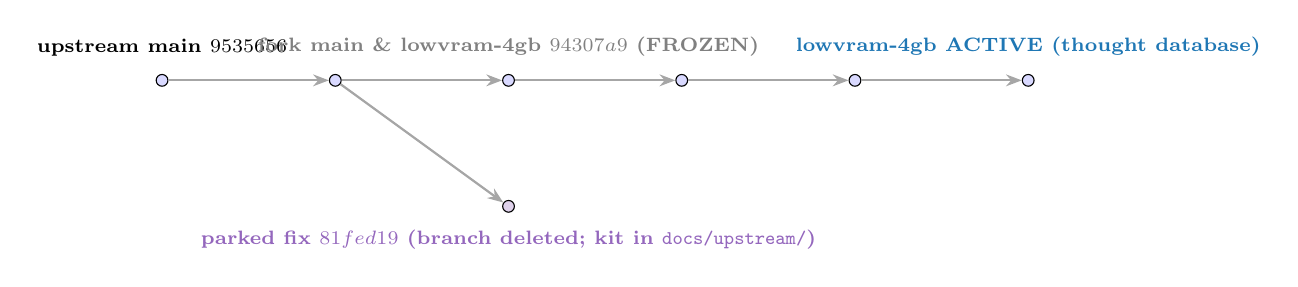
\begin{tikzpicture}[
  commit/.style={draw, circle, fill=blue!15, inner sep=1.5pt, font=\tiny},
  frozen/.style={commit, fill=gray!35},
  parked/.style={commit, fill=park!30},
  ref/.style={font=\scriptsize\bfseries},
  arrow/.style={-{Stealth[length=2mm]}, thick, gray!70}]
\node[commit] (up) at (0,0) {};
\node[ref, above=0.1cm of up] {upstream main $9535656$};
\node[commit] (f1) at (2.2,0) {};
\node[commit] (f2) at (4.4,0) {};
\draw[arrow] (up) -- (f1);
\draw[arrow] (f1) -- (f2);
\node[ref, above=0.1cm of f2, text=gray] {fork main \& lowvram-4gb $94307a9$ (FROZEN)};
\node[commit] (d1) at (6.6,0) {};
\node[commit] (d2) at (8.8,0) {};
\node[commit] (d3) at (11,0) {};
\draw[arrow] (f2) -- (d1);
\draw[arrow] (d1) -- (d2);
\draw[arrow] (d2) -- (d3);
\node[ref, above=0.1cm of d3, text=gpu] {lowvram-4gb ACTIVE (thought database)};
\node[parked] (p1) at (4.4,-1.6) {};
\draw[arrow] (f1) -- (p1);
\node[ref, below=0.1cm of p1, text=park] {parked fix $81fed19$ (branch deleted; kit in \texttt{docs/upstream/})};
\end{tikzpicture}

\medskip
\textbf{Legend:} the fork's \texttt{main} froze at $94307a9$ (upstream + the
8-file 4-GiB patch + docs). All new work — including this thought database —
lands on \texttt{lowvram-4gb}. The upstream bug-fix branch was parked: the
full diff, test, and revival steps live in
\texttt{docs/upstream/PARKED-RESOLVER-DESIGN.md}.

%=====================================================================
\section{Regenerating this document}
%=====================================================================
\begin{tabular}{@{}ll@{}}
\toprule
Action & Command \\
\midrule
Rebuild the PDF & \texttt{make -C docs/visual} \\
Direct latexmk & \texttt{latexmk -pdf -interaction=nonstopmode -halt-on-error} \\
Toolchain & pdflatex + latexmk + tikz/pgfplots (Debian \texttt{texlive-pictures}) \\
Source of truth & this \texttt{.tex}; the committed PDF is a convenience \\
LLM note & the TikZ sources are plain text — fully machine-readable \\
\bottomrule
\end{tabular}

\end{document}
